\chapter{OpenBaton}
\label{ch:ob}

	\section{Configuration requirements}
	\label{sec:Configuration requirements to run OpenBaton on a single server or VM}
	\begin{itemize}
		\item Operating System: Ubuntu 16.04 as base image (\hyperlink{name}{http://releases.ubuntu.com/16.04/})
		\item You will need: Docker (>=18.03) and Docker Compose (>=1.20)
		\item Minimal Version: More than 2GB of RAM, and more than 2 CPUs, 10GB of disk space
		\item Complete Version: More than 8GB of RAM, and more than 8 CPUs, 10GB of disk space
	\end{itemize}

	\section{OpenBaton Installation}
	\label{OpenBaton Installation}
		\paragraph{}
		A minimal version of OpenBaton is installed. Please note that OpenBaton can only be installed on Ubuntu version 16.04 or older. OpenBaton does not provide software package for Ubuntu’s xenial (18.04) version yet. The installation guide can also be found at \hyperlink{name}{https://openbaton.github.io/documentation/nfvo-installation-deb/}. A minimal version comprises of following components.
		\begin{itemize}
			\item Network Function Virtualization Orchestrator (NFVO)
			\item Test Virtual Infrastructure Manager (VIM)
			\item RabbitMQ as messaging system
		\end{itemize}
		\subsection*{Steps of installation:}
		\begin{itemize}
			
			\item Install Curl
			\begin{lstlisting}
sudo apt-get install curl 
			\end{lstlisting}
			
			\item Install components from the Bootstrap repository
			\begin{lstlisting}
sh <(curl -s http://get.openbaton.org/bootstrap) release
			\end{lstlisting}
			
			\item Know your IP Address
			\begin{lstlisting}
curl ifconfig.me
			\end{lstlisting}
			
			\item Quick Start
			\begin{lstlisting}
curl -o docker-compose.yml \ https://raw.githubusercontent.com/openbaton/bootstrap/master/docker-compose.yml | env HOST_IP=$YOUR_LOCAL_IP docker-compose up -d
			\end{lstlisting}
			
			\item Replace YOUR\_LOCAL\_IP with the IP address of your machine. After few seconds check if the OpenBaton dashboard is up and running on https://localhost:8080.
			You can login using following credentials:
			\begin{itemize}
				\item Username: admin
				\item Password: openbaton
			\end{itemize}
		\end{itemize}
			
	\section{Deploy a dummy Network Service}
	\label{Deploy a dummy Network Service}
			\paragraph{}
			Once OpenBaton is installed successfully, the following section lists out steps to deploy a dummy NS which needs following components:
			\begin{itemize}
				\item Network Function Virtualization Orchestrator (NFVO)
				\item Test VIM driver (It does not have to be installed it as it was installed as a part of bootstrap installation)
				\item Dummy Virtual Network Function Manager (Installation steps explained below)
			\end{itemize}
		
			\subsection*{Steps to install dummy VNFM Amqp}
			\begin{itemize}
				
				\item Clone the project
				\begin{lstlisting}
git clone https://github.com/openbaton/dummy-vnfm-amqp.git 
				\end{lstlisting}
				
				\item Switch to the directory where dummy-vnfm-amqp is cloned and compile
				\begin{lstlisting}
cd dummy-vnfm-amqp; ./dummy-vnfm.sh compile
				\end{lstlisting}
				
				\item Start the VNFM
				\begin{lstlisting}
./dummy-vnfm.sh start
java -jar build/libs/dummy-vnfm-amqp-6.0.1-SNAPSHOT.jar
				\end{lstlisting}
				
				\item Start the NFVO with test vim driver
				\begin{itemize}
					\item Download the docker-compose file from \hyperlink{name}{https://openbaton.github.io/documentation/compose/dummy-ns.yml}. This file contains dummy VNFM and test VIM driver.
				\end{itemize}
				\begin{lstlisting}
docker-compose -p ob -f dummy-ns.yml up -d
				\end{lstlisting}
				
				\item Open your browser and navigate to http://localhost:8080 and login to the dashboard
				\item Verify the VNFM of type Dummy is listed under Catalog -> VNF Managers
				\begin{figure} [h]
					\centering
					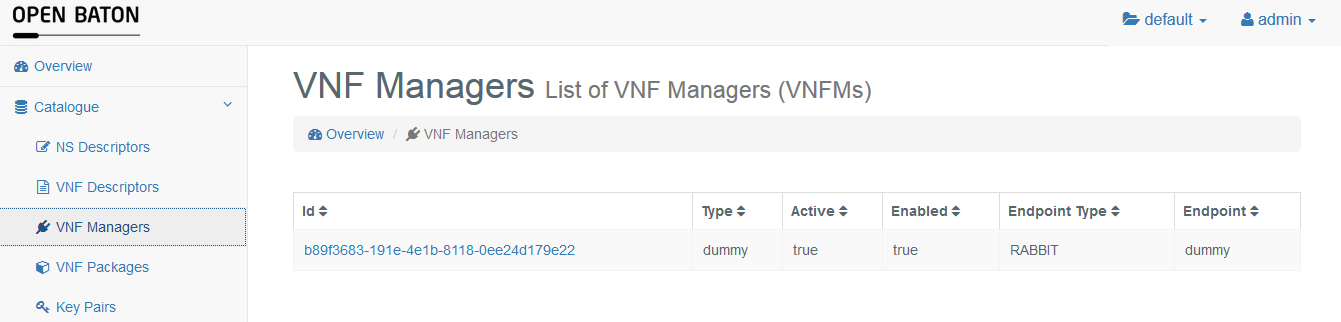
\includegraphics[width=0.7\linewidth]{figures/VNFMList}
					\caption{List of VNF Managers (VNFMs)}
					\label{fig:VNFMList}
				\end{figure}
			\end{itemize}
			
			\subsection*{Deployment of NS using OpenBaton dashboard}
			\paragraph{}
			After installing dummy VNFM the next step is to create a new VIM instance by registering a new Point of Presence using OpenBaton dashboard.
			\begin{itemize}
				\item Register a new PoP
				\begin{itemize}
					\item Open your browser and navigate to http://localhost:8080 and login to the dashboard
					\item Go to Manage PoPs -> PoP Instances -> Register new PoP -> File Input
					\item Upload a VIM instance of type test to the NFVO. Copy paste the JSON content of the link 	\hyperlink{name}{https://openbaton.github.io/documentation/descriptors/vim-instance/test-vim-instance.json}. 
					\begin{figure} [h]
						\centering
						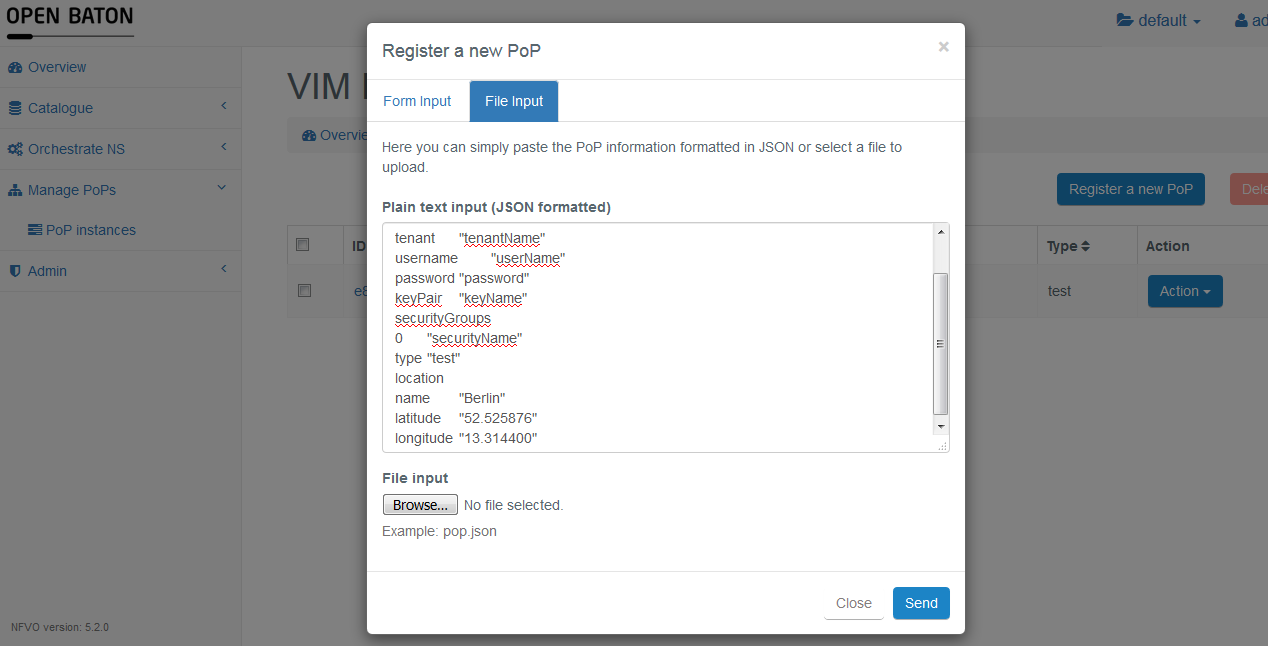
\includegraphics[width=0.7\linewidth]{figures/registerPoP}
						\caption{Register new PoP}
						\label{fig:registerPoP}
					\end{figure}
				\end{itemize}
			
				\item Upload NSD
				\begin{itemize}
					\item Open your browser and navigate to http://localhost:8080 and login to the dashboard
					\item Go to Catalog -> NS Descriptors -> On board NSD -> Upload JSON
					\item Download NSD and upload it. The NSD can be found at \hyperlink{name}{https://openbaton.github.io/documentation/descriptors/tutorial-dummy-NSR/tutorial-dummy-NSR.json}. 
					\begin{figure} [h]
						\centering
						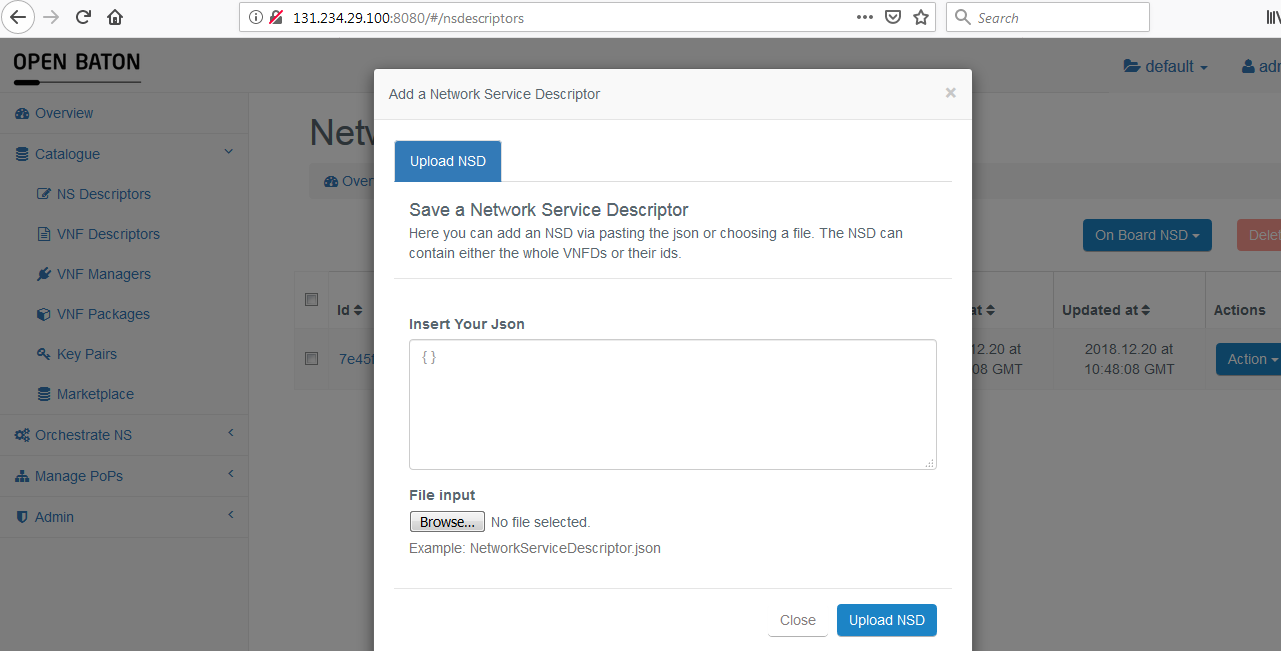
\includegraphics[width=0.7\linewidth]{figures/uploadNSD}
						\caption{Upload NSD}
						\label{fig:uploadNSD}
					\end{figure}
					\item After uploading the NSD, it will be listed under Catalog -> NS Descriptors
					\begin{figure} [h]
						\centering
						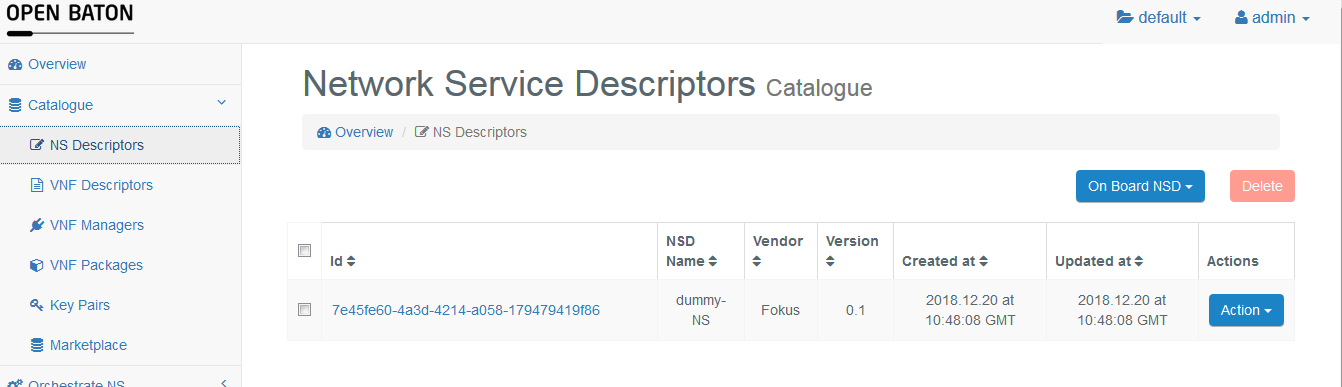
\includegraphics[width=0.7\linewidth]{figures/NSDList}
						\caption{List of NSDs}
						\label{fig:NSDList}
					\end{figure}
					\item Also VNF Descriptors can be seen under Catalog -> VNF Descriptors				
					\begin{figure} [h]
						\centering
						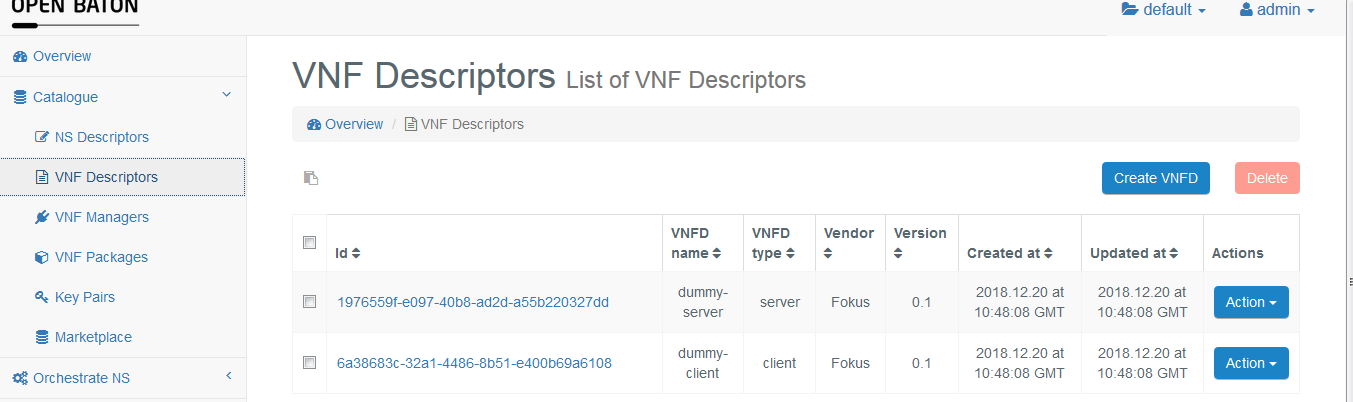
\includegraphics[width=0.7\linewidth]{figures/VNFDList}
						\caption{List of VNFDs}
						\label{fig:VNFDList}
					\end{figure}
				\end{itemize}
			
				\item Deploy NSD
				\begin{itemize}
					\item Open your browser and navigate to http://localhost:8080 and login to the dashboard
					\item After onboarding the NSD in the NFVO , deploy this NSD by using the dashboard.
					\item Goto NS catalogue -> Action -> Launch -> Click Launch again
					\begin{figure} [h]
						\centering
						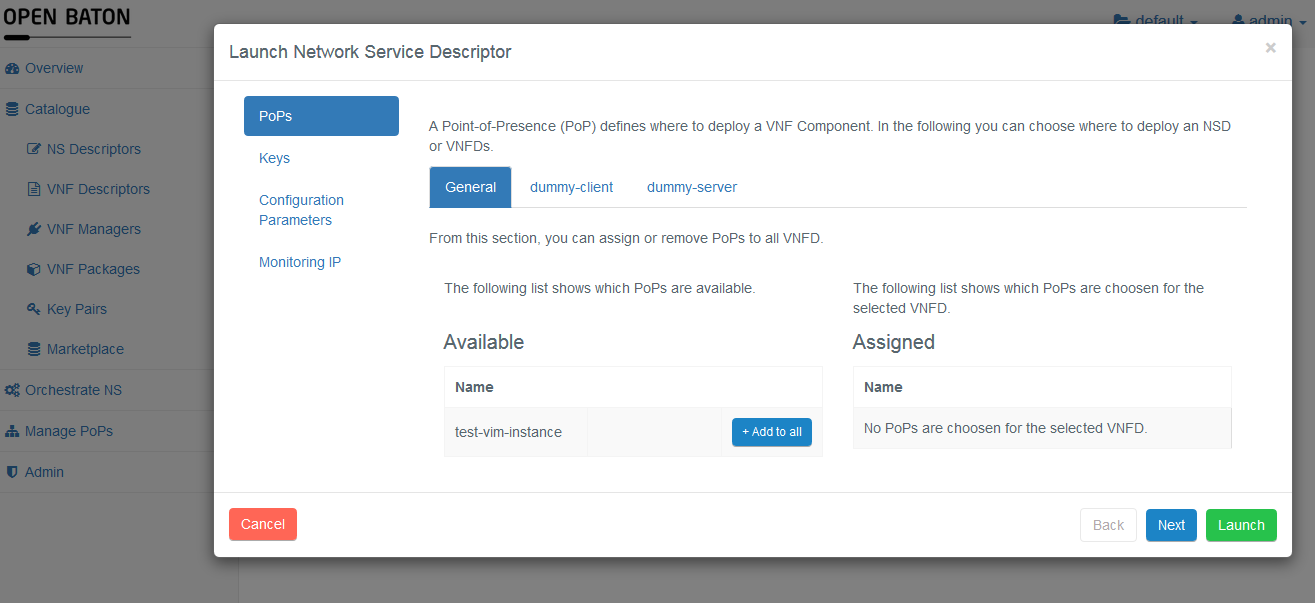
\includegraphics[width=0.7\linewidth]{figures/launchNSD}
						\caption{Upload NSD}
						\label{fig:launchNSD}
					\end{figure}
				\end{itemize}
			
				\item Deploy NSD
				\begin{itemize}
					\item Go to Orchestrate NS -> NS Records
					\item You can see the NS with name dummy-NS and status as Active.
					\begin{figure} [h]
						\centering
						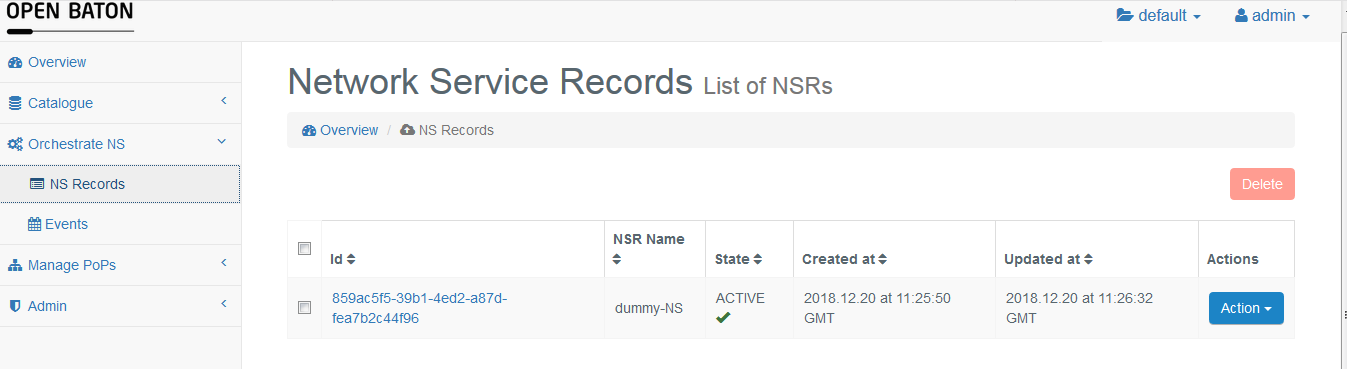
\includegraphics[width=0.7\linewidth]{figures/NSDRecord}
						\caption{Upload NSD}
						\label{fig:NSDRecord}
					\end{figure}
				\end{itemize}
			\end{itemize}